\chapter{Livros e Artigos}
\label{chap:livros e artigos}

\begin{figure}[h!] 
    \captionsetup{width=7cm}%Da mesma largura que a figura
	\Caption{\label{fig:reitoria} Capa do livro: Adapta-se: Por que todo sucesso começa com fracasso.}
	\UFCfig{}{
		\includegraphics[width=7cm]{figuras/adapt-hb-uk.png}
	}{
		\Fonte{Web Site: TimHardford.com}
	}	
\end{figure}

Adapta-se: Por que todo sucesso começa com fracasso.
Adaptar-se propões uma abordagem surpreendente para aceitar o fracasso como parte do processo de inovação
Altas expectativas podem gerar altas decepções quando as previsões dão errado.
Burocracia e autoridade retêm processos de inovação
Incentivar e dar mérito pode impulsionar a inovação e o crescimento

Adapt Neste livro inovador, Tim Harford, o Economista Disfarçado, nos mostra uma nova e inspiradora abordagem para resolver os problemas mais urgentes de nossas vidas. Diante de situações complexas, todos nós nos acostumamos a olhar para nossos líderes para definir um plano de ação e abrir um caminho para o sucesso. Harford argumenta que os desafios de hoje simplesmente não podem ser enfrentados com soluções prontas e opinião de especialistas; o mundo tornou-se muito imprevisível e profundamente complexo. Em vez disso, devemos nos adaptar.

Tecendo habilmente psicologia, biologia evolutiva, antropologia, física e economia, juntamente com a história convincente de lições duramente conquistadas aprendidas no campo, Harford faz um caso apaixonado pela importância da tentativa adaptativa e do erro no enfrentamento de questões como mudanças climáticas, pobreza e crises financeiras - bem como no fomento à inovação e criatividade em nossos negócios e vidas pessoais.

Nos levando das salas de reuniões corporativas para os desertos do Iraque, Adapt explica claramente os ingredientes necessários para transformar o fracasso em sucesso. É um manual inovador para sobreviver e prosperar em nosso complexo e sempre em mudança.

\begin{figure}[h!] 
    \captionsetup{width=7cm}%Da mesma largura que a figura
	\Caption{\label{fig:reitoria} Capa do livro: O Economista disfarçado}
	\UFCfig{}{
		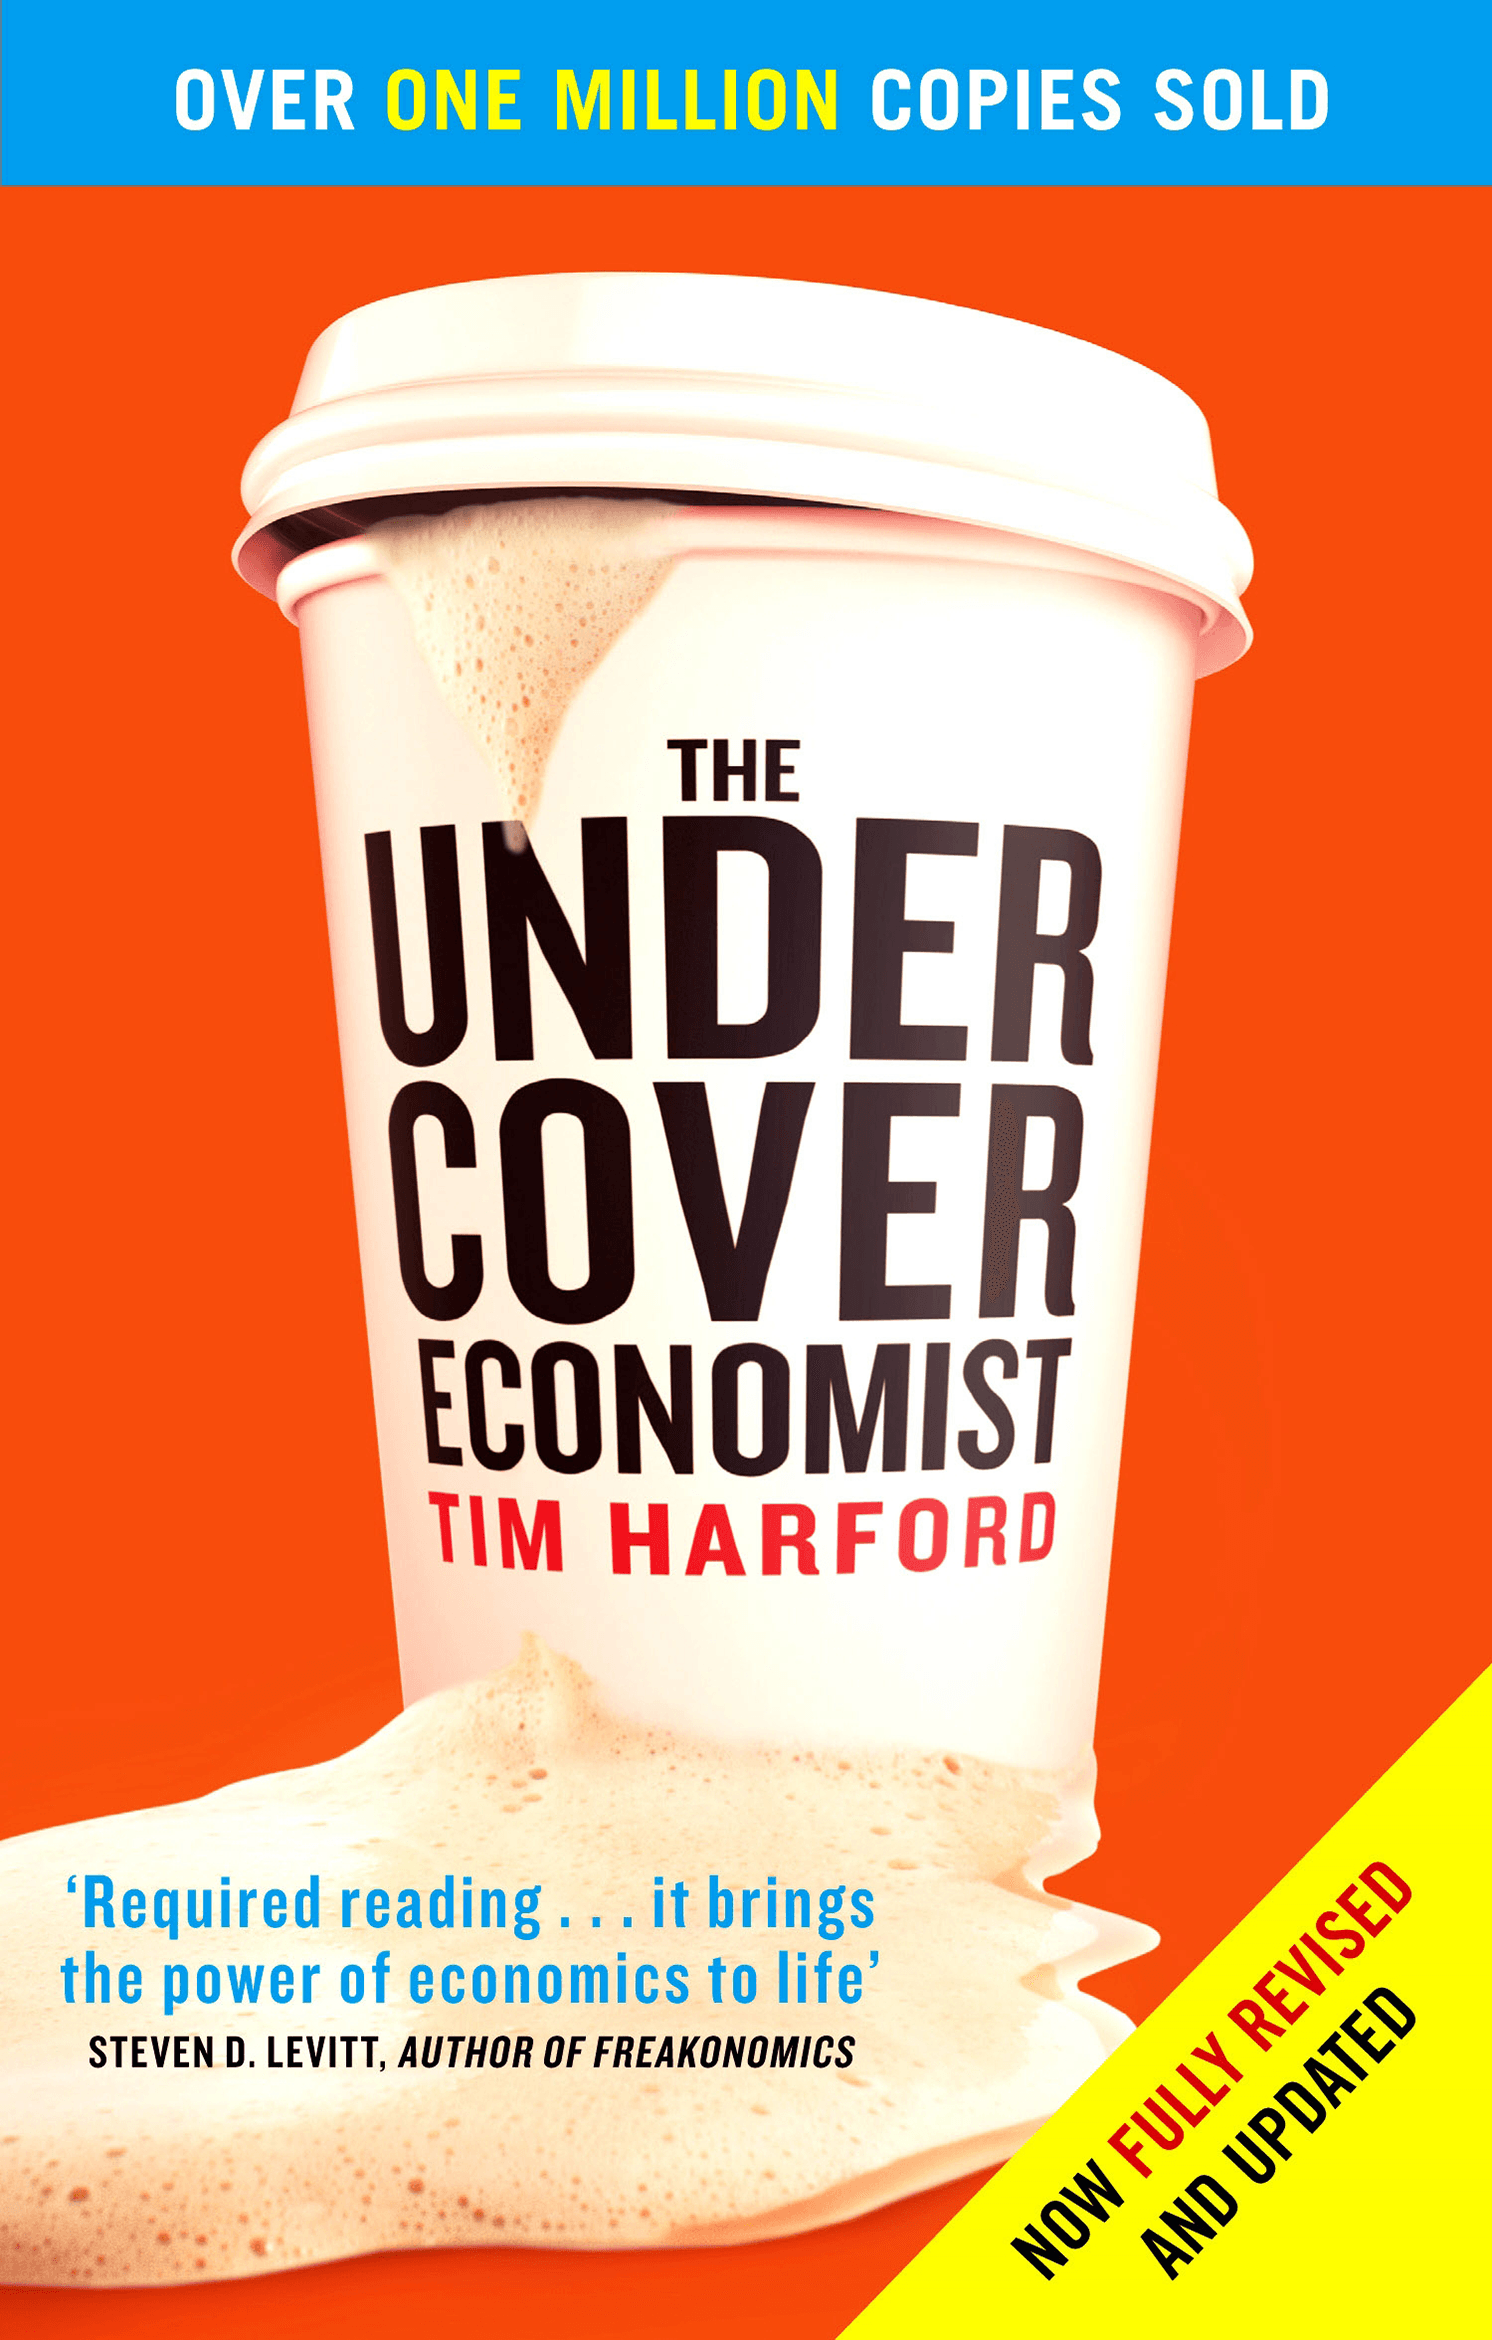
\includegraphics[width=7cm]{figuras/the-undercover-economist.png}
	}{
		\Fonte{Web Site: TimHardford.com}
	}	
\end{figure}

Livro The Undercover Economist 
A versão de um economista de como as coisas funcionam, este volume envolvente é guia de campo parte para a economia ea parte expor os princípios econômicos à espreita por trás dos eventos diários, explicando tudo, desde engarrafamentos aos preços elevados do café. The Economist secreta é para quem está se perguntou por que o fosso entre países ricos e pobres é tão grande, ou porque não consigo encontrar um carro em segunda mão decente, ou como enganar Starbucks. Este livro oferece a história escondida por trás destas e de outras questões, como o economista Tim Harford varia de África, Ásia, Europa, e, claro, os Estados Unidos para revelar como supermercados, companhias aéreas e cadeias de café - para citar apenas alguns - são aspiração dinheiro de nossas carteiras. Harford perfura os mitos que cercam alguns dos maiores controvérsias de hoje, incluindo o alto custo dos cuidados de saúde; ele revela por que certas leis ambientais pode colocar um sorriso no rosto de um proprietário; e ele explica por que algumas indústrias podem ter altos lucros por razões inocentes, enquanto em outras indústrias algo sinistro está acontecendo. Cobrindo uma gama de conceitos econômicos, incluindo os escassos recursos, poder de mercado, eficiência, manipulação de preços, falha de mercado, informação privilegiada e teoria dos jogos, Harford lança luz sobre como essas forças moldar nossas vidas do dia-a-dia, muitas vezes sem o nosso conhecimento. Mostrando-nos o mundo através dos olhos de um economista, Tim Harford revela que eventos diários são jogos intrincados de negociações, concursos de força e batalhas de inteligência. Escrito com um leve toque e sagacidade manhoso, The Economist disfarçado transforma "a ciência desânimo" em um verdadeiro deleite.

\begin{figure}[h!] 
    \captionsetup{width=7cm}%Da mesma largura que a figura
	\Caption{\label{fig:reitoria} Capa do livro: Próximas cinquentas coisas}
	\UFCfig{}{
		\includegraphics[width=7cm]{figuras/next50things.png}
	}{
		\Fonte{Web Site: TimHardford.com}
	}	
\end{figure}

 

Livro Next Fifty Things 
Em Cinquenta Coisas que Fizeram a Economia Moderna, o revolucionário e aclamado livro, séries de rádio e podcast, o economista best-seller Tim Harford nos apresentou uma seleção de cinquenta invenções radicais que mudaram o mundo.

Agora, neste novo livro, Harford mais uma vez nos traz uma série de "coisas" notáveis, memoráveis, curiosas e muitas vezes inesperadas - invenções que nos ensinam lições por turnos íntimos e arrebatadores sobre a complexa economia mundial em que vivemos hoje.

Do tijolo, blockchain e da bicicleta ao fogo, da fábrica e da captação de recursos, e da solar fotovoltaica e do lápis ao selo postal, essa coleção brilhante e esclarecedora ressoa, fascina e estimula. É uma maravilhosa mistura de perspicácia e inspiração de um dos melhores contadores de histórias de não-ficção da Grã-Bretanha.

\section{Viés do empreendedorismo}\label{sec:exemplo-de-algoritmos-e-figuras}
Economia Criativa
Como a economia produziu todas essas coisas incríveis que temos ao nosso redor - computadores e telefones celulares e assim por diante? Havia um monte de idéias, e os bons cresceram e prosperaram. E os maus eram muito impiedosamente eliminados.

Objetivo é criar uma rede de artistas e empresários que tenham a capacidade de promover um crescimento sustentável no setor criativo valorizando a criatividade individual ou coletiva, habilidades e talentos.
Empresas com esse segmento exemplos: Quinto Andar, Canguru, ABlab, Nós Todos Filmes, Aram e Even3


\section{Artigos}
\label{sec:Artigos}

Tim Hardford publico semanalmente artigos no jornal onde ele trabalha, no Finacial Times, na qual ele abordagens váriados temas, principalmente sobre economia, mas também outros temas como filosofia, finanças, saúde entre outros. Aqui estão alguns exemplos.

A ilusão de crescimento de  Liz Truss 

Quanto dinheiro vai te fazer feliz?

Mesmo quando você consegue, às vezes vale a pena tentar de novo

Aborto e mulheres na América: o que os números dizem?

